\documentclass[../psets.tex]{subfiles}

\pagestyle{main}
\renewcommand{\leftmark}{Problem Set \thesection}

\begin{document}




\section{The Kinetic Theory of Gases}
\emph{From \textcite{bib:McQuarrieSimon}.}
\subsection*{Chapter 27}
\begin{enumerate}[label={\textbf{27-\arabic*.}},leftmargin=3.5em]
    \setcounter{enumi}{4}
    \item Arrange the following gases in order of increasing root-mean-square speed at the same temperature: \ce{O2}, \ce{N2}, \ce{H2O}, \ce{CO2}, \ce{NO2}, \ce{{}^235UF6}, \ce{{}^238UF6}.
    \begin{proof}[Answer]
        The root mean square speed is given by
        \begin{equation*}
            u_\text{rms} = \sqrt{\frac{3RT}{M}}
        \end{equation*}
        Thus, since the temperature is constant by hypothesis, the root mean square speed ordering will be entirely a function of the molar mass (and inversely proportional to it at that). It follows since
        \begin{align*}
            M(\ce{O2})        &= \SI[per-mode=symbol]{32.00}{\gram\per\mole}\\
            M(\ce{N2})        &= \SI[per-mode=symbol]{38.02}{\gram\per\mole}\\
            M(\ce{H2O})       &= \SI[per-mode=symbol]{18.02}{\gram\per\mole}\\
            M(\ce{CO2})       &= \SI[per-mode=symbol]{44.01}{\gram\per\mole}\\
            M(\ce{NO2})       &= \SI[per-mode=symbol]{46.01}{\gram\per\mole}\\
            M(\ce{{}^235UF6}) &= \SI[per-mode=symbol]{349.08}{\gram\per\mole}\\
            M(\ce{{}^238UF6}) &= \SI[per-mode=symbol]{352.04}{\gram\per\mole}
        \end{align*}
        that
        \begin{equation*}
            \boxed{
                u_\text{rms}(\ce{{}^238UF6}) < u_\text{rms}(\ce{{}^235UF6})
                < u_\text{rms}(\ce{NO2})
                < u_\text{rms}(\ce{CO2})
                < u_\text{rms}(\ce{N2})
                < u_\text{rms}(\ce{O2})
                < u_\text{rms}(\ce{H2O})
            }
        \end{equation*}
    \end{proof}
    \stepcounter{enumi}
    \item The speed of sound in an ideal monatomic gas is given by
    \begin{equation*}
        u_\text{sound} = \sqrt{\frac{5RT}{3M}}
    \end{equation*}
    Derive an equation for the ratio $u_\text{rms}/u_\text{sound}$. Calculate the root-mean-square speed for an argon atom at \SI{20}{\celsius} and compare your answer to the speed of sound in argon.
    \begin{proof}[Answer]
        We have that
        \begin{align*}
            \frac{u_\text{rms}}{u_\text{sound}} &= \frac{\sqrt{3RT/M}}{\sqrt{5RT/3M}}\\
            \Aboxed{\frac{u_\text{rms}}{u_\text{sound}} &= \sqrt{9/5}}
        \end{align*}
        The root mean square speed for an argon atom at \SI{20}{\celsius} is given by
        \begin{align*}
            u_\text{rms}(\ce{Ar}) &= \sqrt{\frac{3(\SI[per-mode=fraction]{8.31}{\joule\per\mole\per\kelvin})(\SI{293}{\kelvin})}{\SI[per-mode=fraction]{0.03995}{\kilo\gram\per\mole}}}\\
            \Aboxed{u_\text{rms}(\ce{Ar}) &= \SI[per-mode=symbol]{428}{\meter\per\second}}
        \end{align*}
        Similarly, the speed of sound in argon at \SI{20}{\celsius} is given by
        \begin{align*}
            u_\text{sound}(\ce{Ar}) &= \sqrt{\frac{5(\SI[per-mode=fraction]{8.31}{\joule\per\mole\per\kelvin})(\SI{293}{\kelvin})}{3(\SI[per-mode=fraction]{0.03995}{\kilo\gram\per\mole})}}\\
            \Aboxed{u_\text{sound}(\ce{Ar}) &= \SI[per-mode=symbol]{319}{\meter\per\second}}
        \end{align*}
        and thus that
        \begin{equation*}
            \frac{u_\text{rms}(\ce{Ar})}{u_\text{sound}(\ce{Ar})} = \frac{\SI[per-mode=symbol]{428}{\meter\per\second}}{\SI[per-mode=symbol]{319}{\meter\per\second}}
            = 1.34
            \approx \sqrt{9/5}
        \end{equation*}
        as desired.
    \end{proof}
    \setcounter{enumi}{11}
    \item We can use the equation for $f(u_x)$ to calculate the probability that the $x$-component of the velocity of a molecule lies within some range. For example, show that the probability that $-u_{x0}\leq u_x\leq u_{x0}$ is given by
    \begin{align*}
        \Prob\{-u_{x0}\leq u_x\leq u_{x0}\} &= \sqrt{\frac{m}{2\pi\kB T}}\int_{-u_{x0}}^{u_{x0}}\e[-mu_x^2/2\kB T]\dd{u_x}\\
        &= 2\sqrt{\frac{m}{2\pi\kB T}}\int_0^{u_{x0}}\e[-mu_x^2/2\kB T]\dd{u_x}
    \end{align*}
    Now let $mu_x^2/2\kB T=w^2$ to get the cleaner looking expression
    \begin{equation*}
        \Prob\{-u_{x0}\leq u_x\leq u_{x0}\} = \frac{2}{\sqrt{\pi}}\int_0^{w_0}\e[-w^2]\dd{w}
    \end{equation*}
    where $w_0=u_{x0}\sqrt{m/2\kB T}$.\par
    It so happens that the above integral cannot be evaluated in terms of any function that we have encountered up to now. It is customary to express the integral in terms of a new function called the \textbf{error function}, which is defined by
    \begin{equation*}
        \erf(z) = \frac{2}{\sqrt{\pi}}\int_0^z\e[-x^2]\dd{x}
    \end{equation*}
    The error function can be evaluated as a function of $z$ by evaluating its defining integral numerically. Some values of $\erf(z)$ are
    \begin{center}
        \small
        \renewcommand{\arraystretch}{1.4}
        \begin{tabular}{cc|cc}
            $z$ & $\erf(z)$ & $z$ & $\erf(z)$\\
            \hline
            0.20 & 0.22270 & 1.20 & 0.91031\\
            0.40 & 0.42839 & 1.40 & 0.95229\\
            0.60 & 0.60386 & 1.60 & 0.97635\\
            0.80 & 0.74210 & 1.80 & 0.98909\\
            1.00 & 0.84270 & 2.00 & 0.99532\\
        \end{tabular}
    \end{center}
    Now show that
    \begin{equation*}
        \Prob\{-u_{x0}\leq u_x\leq u_{x0}\} = \erf(w_0)
    \end{equation*}
    Calculate the probability that $-\sqrt{2\kB T/m}\leq u_x\leq\sqrt{2\kB T/m}$.
    \begin{proof}[Answer]
        The probability distribution $f(u_x)$ of the $x$-components of the velocity of a system of molecules is given by
        \begin{equation*}
            f(u_x) = \sqrt{\frac{m}{2\pi\kB T}}\e[-mu_x^2/2\kB T]
        \end{equation*}
        It follows that the probability that the $x$-component of the velocity of a molecule lies between $u_x$ and $u_x+\dd{u_x}$ is $f(u_x)\dd{u_x}$. Thus, to calculate the total probability that the $x$-component of the velocity of a molecule lies within the range $-u_{x0}\leq u_x\leq u_{x0}$, we can use an integral to sum all of the infinitesimal probabilities $f(u_x)\dd{u_x}$ in that range as follows.
        \begin{align*}
            \Prob\{-u_{x0}\leq u_x\leq u_{x0}\} &= \int_{-u_{x0}}^{u_{x0}}f(u_x)\dd{u_x}\\
            &= \sqrt{\frac{m}{2\pi\kB T}}\int_{-u_{x0}}^{u_{x0}}\e[-mu_x^2/2\kB T]\dd{u_x}\\
            &= 2\sqrt{\frac{m}{2\pi\kB T}}\int_0^{u_{x0}}\e[-mu_x^2/2\kB T]\dd{u_x}
        \end{align*}
        Note that the last equality holds because $f(u_x)=g(u_x^2)$, where $u_x^2$ is an even function and hence $f$ is even. Now define the function $w(u_x)$ by
        \begin{equation*}
            w^2 = \frac{mu_x^2}{2\kB T}
        \end{equation*}
        Since $w$ is monotonically increasing on the range $[0,u_{x0}]$, and
        \begin{align*}
            w(0) &= 0&
                w(u_{x0}) &= u_{x0}\sqrt{\frac{m}{2\kB T}}&
                    2w\dv{w}{u_x} &= \frac{2mu_x}{2\kB T}\\
            &&
                &&
                    \frac{2w\kB T}{mu_x}\dd{w} &= \dd{u_x}\\
            &&
                &&
                    \frac{2u_x\sqrt{m/2\kB T}\kB T}{mu_x}\dd{w} &= \dd{u_x}\\
            &&
                &&
                    \sqrt{\frac{2\kB T}{m}}\dd{w} &= \dd{u_x}
        \end{align*}
        we may substitute it into the above integral using the $u$-substitution method to yield
        \begin{align*}
            \Prob\{-u_{x0}\leq u_x\leq u_{x0}\} &= 2\sqrt{\frac{m}{2\pi\kB T}}\cdot\sqrt{\frac{2\kB T}{m}}\int_{w(0)}^{w(u_{x0})}\e[-w^2]\dd{w}\\
            &= \frac{2}{\sqrt{\pi}}\int_{0}^{w_0}\e[-w^2]\dd{w}
        \end{align*}
        Naturally, the above equals $\erf(w_0)$ by the definition of the error function.\par
        Lastly, if $u_{x0}=\sqrt{2\kB T/m}$, then
        \begin{equation*}
            w_0 = u_{x0}\sqrt{m/2\kB T}
            = \sqrt{2\kB T/m}\cdot\sqrt{m/2\kB T}
            = 1
        \end{equation*}
        It follows that
        \begin{align*}
            \Prob\{-\sqrt{2\kB T/m}\leq u_x\leq\sqrt{2\kB T/m}\} &= \erf(w_0)\\
            &= \erf(1)\\
            \Aboxed{\Prob\{-\sqrt{2\kB T/m}\leq u_x\leq\sqrt{2\kB T/m}\} &= 0.84270}
        \end{align*}
    \end{proof}
    \setcounter{enumi}{19}
    \item Show that the variance of the equation $I(\nu)\propto\e[-mc^2(\nu-\nu_0)^2/2\nu_0^2\kB T]$ is given by $\sigma^2=\nu_0^2\kB T/mc^2$. Calculate $\sigma$ for the $3p$ ${}^2P_{3/2}$ to $3s$ ${}^2S_{1/2}$ transition in atomic sodium vapor (see Figure 8.4 on \textcite[307]{bib:McQuarrieSimon}) at \SI{500}{\kelvin}.
    \begin{proof}[Answer]
        As per MathChapter B of \textcite{bib:McQuarrieSimon}, $I(\nu)$ is a Gaussian distribution, i.e., is of the form $\e[-(x-\prb{x})^2/2\sigma^2]$ where $\sigma$ is the standard deviation. It follows by comparing this general form with the given equation for $I(\nu)$ that
        \begin{equation*}
            \sigma^2 = \frac{\nu_0^2\kB T}{mc^2}
        \end{equation*}
        From Figure 8.4, we have that
        \begin{equation*}
            \lambda(3p\ {}^2P_{3/2}\to 3s\ {}^2S_{1/2}) = \SI{5.8899e3}{\angstrom}
        \end{equation*}
        Thus,
        \begin{equation*}
            \nu_0 = \frac{c}{\lambda}
            = \frac{\SI{2.998e8}{\meter\per\second}}{\SI{5.8899e-7}{\meter}}
            = \SI{5.090e14}{\per\second}
        \end{equation*}
        Therefore, we have that
        \begin{align*}
            \sigma &= \sqrt{\frac{\nu_0^2RT}{Mc^2}}\\
            &= \sqrt{\frac{(\SI[per-mode=fraction]{5.090e14}{\per\second})^2(\SI[per-mode=fraction]{8.31}{\joule\per\mole\per\kelvin})(\SI{500}{\kelvin})}{(\SI[per-mode=fraction]{0.02299}{\kilo\gram\per\mole})(\SI[per-mode=fraction]{2.998e8}{\meter\per\second})^2}}\\
            \Aboxed{\sigma &= \SI{7.22e8}{\per\second}}
        \end{align*}
    \end{proof}
    \setcounter{enumi}{23}
    \item Show that the probability that a molecule has a speed less than or equal to $u_0$ is given by
    \begin{equation*}
        \Prob\{u\leq u_0\} = \frac{4}{\sqrt{\pi}}\int_0^{x_0}x^2\e[-x^2]\dd{x}
    \end{equation*}
    where $x_0=u_0\sqrt{m/2\kB T}$. This integral cannot be expressed in terms of any known function and must be integrated numerically. Use Simpson's rule or any other integration routine to evaluate $\Prob\{u\leq\sqrt{2\kB T/m}\}$.
    \begin{proof}[Answer]
        As in Problem 27-12, we have that
        \begin{align*}
            \Prob\{u\leq u_0\} &= \int_0^{u_0}F(u)\dd{u}\\
            &= 4\pi\left( \frac{m}{2\pi\kB T} \right)^{3/2}\int_0^{u_0}u^2\e[-mu^2/2\kB T]\dd{u}\\
            &= 4\pi\left( \frac{m}{2\pi\kB T} \right)^{3/2}\cdot\sqrt{\frac{2\kB T}{m}}\int_{x(0)}^{x(u_0)}\frac{2\kB Tx^2}{m}\e[-x^2]\dd{x}\\
            &= 4\pi\left( \frac{m}{2\pi\kB T} \right)^{3/2}\cdot\left( \frac{2\kB T}{m} \right)^{1/2}\cdot\left( \frac{2\kB T}{m} \right)\int_0^{x_0}x^2\e[-x^2]\dd{x}\\
            &= \frac{4}{\sqrt{\pi}}\int_0^{x_0}x^2\e[-x^2]\dd{x}
        \end{align*}
        We now evaluate
        \begin{equation*}
            \Prob\{u\leq\sqrt{2\kB T/m}\} = \frac{4}{\sqrt{\pi}}\int_0^1x^2\e[-x^2]\dd{x}
        \end{equation*}
        using Simpson's rule with four subdivisions, each having height $h=0.25$, as follows.
        \begin{align*}
            \Prob\{u\leq\sqrt{2\kB T/m}\} &\approx \frac{0.25}{3}[g(0)+4g(0.25)+2g(0.5)+4g(0.75)+g(1)]\\
            &= \frac{1}{12}(0+4\cdot 0.059+2\cdot 0.195+4\cdot 0.321+0.367)\\
            \Aboxed{\Prob\{u\leq\sqrt{2\kB T/m}\} &\approx 0.190}
        \end{align*}
    \end{proof}
    \setcounter{enumi}{26}
    \item Derive an expression for $\sigma_\varepsilon^2=\prb{\varepsilon^2}-\prb{\varepsilon}^2$ from the equation for $F(\varepsilon)\dd{\varepsilon}$. Now form the ratio $\sigma_\varepsilon/\prb{\varepsilon}$. What does this say about the fluctuation in $\varepsilon$?
    \begin{proof}[Answer]
        We know from class that
        \begin{equation*}
            \prb{\varepsilon} = \frac{3}{2}\kB T
        \end{equation*}
        Additionally, we can derive that
        \begin{align*}
            \prb{\varepsilon^2} &= \int_0^\infty\varepsilon^2F(\varepsilon)\dd{\varepsilon}\\
            &= \frac{2\pi}{(\pi\kB T)^{3/2}}\int_0^\infty\varepsilon^2\cdot\varepsilon^{1/2}\e[-\varepsilon/\kB T]\dd{\varepsilon}\\
            &= \frac{2\pi}{(\pi\kB T)^{3/2}}\int_0^\infty\varepsilon^{5/2}\e[-\varepsilon/\kB T]\dd{\varepsilon}\\
            &= \frac{2\pi}{(\pi\kB T)^{3/2}}\cdot\frac{15}{8}\left[ \pi(\kB T)^7 \right]^{1/2}\\
            &= \frac{15}{4}(\kB T)^2
        \end{align*}
        Thus, we have that
        \begin{align*}
            \sigma_\varepsilon^2 &= \prb{\varepsilon^2}-\prb{\varepsilon}^2\\
            &= \frac{15}{4}(\kB T)^2-\frac{9}{4}(\kB T)^2\\
            \Aboxed{\sigma_\varepsilon^2 &= \frac{2}{3}(\kB T)^2}
        \end{align*}
        Taking
        \begin{equation*}
            \frac{\sigma_\varepsilon}{\prb{\varepsilon}} = \frac{\sqrt{2/3}\kB T}{3\kB T/2}
            = \left( \frac{2}{3} \right)^{3/2}
        \end{equation*}
        reveals that the fluctuation in $\varepsilon$ is sizeable with respect to the average energy.
    \end{proof}
    \setcounter{enumi}{33}
    \item The figure below illustrates another method that has been used to determine the distribution of molecular speeds.
    \begin{figure}[H]
        \centering
        \footnotesize
        \begin{subfigure}[b]{0.49\linewidth}
            \centering
            \begin{tikzpicture}[
                every path/.style={semithick}
            ]
                \path (-4,0) -- (4,0);
    
                \draw circle (2cm);
                \draw [double=white,double distance=1mm] (-2.1,0) -- (-1.9,0);
                \draw [white,line width=1mm] (-2.2,0) -- (-1.8,0);
    
                \draw [-latex] (0,0) -- node[below right=-2pt]{$R$} (45:2);
                \draw [-latex] (-2.5,0) node[left,align=center]{Pulse of\\molecules} -- (-1.5,0);
                \draw [decorate,decoration={text along path,text=Direction of drum rotation}] (120:2.2) arc[start angle=120,end angle=-90,radius=2.2cm];
                \draw [-latex] (123:2.28) arc[start angle=123,end angle=150,radius=2.28cm];
            \end{tikzpicture}
            \caption{}
        \end{subfigure}
        \begin{subfigure}[b]{0.3\linewidth}
            \centering
            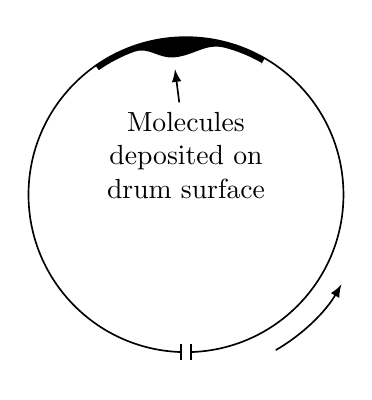
\begin{tikzpicture}[
                every path/.style={semithick}
            ]
                \draw circle (2cm);
                \draw [double=white,double distance=1mm] (-90:2.1) -- (-90:1.9);
                \draw [white,line width=1mm] (-90:2.2) -- (-90:1.8);
    
                \fill (60:1.9)
                    -- (60:2)
                    arc[start angle=60,end angle=125,radius=2cm]
                    -- (125:1.93)
                    arc[start angle=125,end angle=110,radius=1.93cm]
                    to[out=20,in=-175] (95:1.75)
                    to[out=5,in=165] (75:1.93)
                    arc[start angle=75,end angle=60,radius=1.93cm]
                    -- cycle
                ;
                \node [align=center] at (0,0.5) {Molecules\\deposited on\\drum surface}
                    edge [-latex] (95:1.6);
                ;
    
                \draw [-latex] (-60:2.28) arc[start angle=-60,end angle=-30,radius=2.28cm];
            \end{tikzpicture}
            \caption{}
        \end{subfigure}
    \end{figure}
    A pulse of molecules collimated from a hot oven enters a rotating hollow drum. Let $R$ be the radius of the drum, $\nu$ be the rotational frequency, and $s$ be the distance through which the drum rotates during the time it takes for a molecule to travel from the entrance slit to the inner surface of the drum. Show that
    \begin{equation*}
        s = \frac{4\pi R^2\nu}{u}
    \end{equation*}
    where $u$ is the speed of the molecule.\par
    Use the equation for $\dd{z_\text{coll}}$ to show that the distribution of molecular speeds emerging from the over is proportional to $u^3\e[-mu^2/2\kB T]\dd{u}$. Now show that the distribution of molecules striking the inner surface of the cylinder is given by
    \begin{equation*}
        I(s)\dd{s} = \frac{A}{s^5}\e[-m(4\pi R^2\nu)^2/2\kB Ts^2]\dd{s}
    \end{equation*}
    where $A$ is simply a proportionality constant. Plot $I$ versus $s$ for various values of $4\pi R^2\nu/\sqrt{2\kB T/m}$, say 0.1, 1, and 3. Experimental data are quantitatively described by the above equation.
    \begin{proof}[Answer]
        Once the molecule enters the drum, it must travel a distance $2R$ before striking the opposite side. It will cover this distance in $2R/u$ seconds. Moreover, we know that the drum rotates once every $\nu$ seconds, so the drum will perform $2R\nu/u$ of a rotation in $2R/u$ seconds. Finally, since a point on the inner surface of the drum moves a distance of $2\pi R$ with every rotation, the inner surface of the drum will move a distance
        \begin{equation*}
            s = \frac{4\pi R^2\nu}{u}
        \end{equation*}
        over the course of the molecule's trip across the interior of the drum. Succinctly,
        \begin{equation*}
            s = \frac{2R\text{ meters}}{1}\times\frac{1\text{ second}}{u\text{ meters}}\times\frac{\nu\text{ rotations}}{1\text{ second}}\times\frac{2\pi R\text{ meters}}{1\text{ rotation}}
            = \frac{4\pi R^2\nu}{u}
        \end{equation*}
        The equation for $\dd{z_\text{coll}}$ describes the collision frequency of atoms moving in a single direction with a single speed. Since the atoms leave the oven in a single direction, the only variable factor on which $\dd{z_\text{coll}}$ depends is $uF(u)\dd{u}\propto u^3\e[-mu^2/2\kB T]\dd{u}$, as desired.\par
        Let $I(u)\dd{u}$ be the distribution of molecules that strike the inner surface of the cylinder with speed between $u$ and $u+\dd{u}$. By the above,
        \begin{equation*}
            I(u)\dd{u} \propto u^3\e[-mu^2/2\kB T]\dd{u}
        \end{equation*}
        Since we have that
        \begin{align*}
            u &= \frac{4\pi R^2\nu}{s}&
            \dd{u} &= -\frac{4\pi R^2\nu}{s^2}\dd{s}
        \end{align*}
        we know that
        \begin{equation*}
            I(s)\dd{s} \propto \left( \frac{4\pi R^2\nu}{s} \right)^3\e[-m(4\pi R^2\nu/s)^2/2\kB T]\cdot -\frac{4\pi R^2\nu}{s^2}\dd{s}
            = \frac{A}{s^5}\e[-m(4\pi R^2\nu)^2/2\kB Ts^2]\dd{s}
        \end{equation*}
        where we have incorporated all external constants into the proportionality constant $A$.\par
        The following are the desired plots
        \begin{figure}[h!]
            \centering
            \begin{subfigure}[b]{0.3\linewidth}
                \centering
                \begin{tikzpicture}
                    \small
                    \draw [stealth-stealth] (0,1.5) -- node[left=13mm]{$I$} (0,0) -- node[below=5mm]{$s$} (2.5,0);
            
                    \footnotesize
                    \draw (1,0.1) -- ++(0,-0.2) node[below]{1};
                    \draw (2,0.1) -- ++(0,-0.2) node[below]{2};
                    \draw (0.1,1) -- ++(-0.2,0) node[left]{\num{100000}};
            
                    \draw [rex,thick] plot[domain=0.01:1.9,smooth,samples=100,/pgf/fpu,/pgf/fpu/output format=fixed] (\x,{1/(\x)^5/100000*e^(-0.01/(\x)^2)});
                \end{tikzpicture}
                \caption{0.1}
            \end{subfigure}
            \begin{subfigure}[b]{0.3\linewidth}
                \centering
                \begin{tikzpicture}
                    \small
                    \draw [stealth-stealth] (0,1.5) -- node[left=5mm]{$I$} (0,0) -- node[below=5mm]{$s$} (2.5,0);
            
                    \footnotesize
                    \draw (1,0.1) -- ++(0,-0.2) node[below]{1};
                    \draw (2,0.1) -- ++(0,-0.2) node[below]{2};
                    \draw (0.1,1) -- ++(-0.2,0) node[left]{1};
            
                    \draw [rex,thick] plot[domain=0.01:1.9,smooth,samples=100,/pgf/fpu,/pgf/fpu/output format=fixed] (\x,{1/(\x)^5*e^(-1/(\x)^2)});
                \end{tikzpicture}
                \caption{1}
            \end{subfigure}
            \begin{subfigure}[b]{0.3\linewidth}
                \centering
                \begin{tikzpicture}
                    \small
                    \draw [stealth-stealth] (0,1.5) -- node[left=10mm]{$I$} (0,0) -- node[below=5mm]{$s$} (2.5,0);
            
                    \footnotesize
                    \draw (1,0.1) -- ++(0,-0.2) node[below]{1};
                    \draw (2,0.1) -- ++(0,-0.2) node[below]{2};
                    \draw (0.1,1) -- ++(-0.2,0) node[left]{\num{0.01}};
            
                    \draw [rex,thick] plot[domain=0.01:1.9,smooth,/pgf/fpu,/pgf/fpu/output format=fixed] (\x,{1/(\x)^5*100*e^(-9/(\x)^2)});
                \end{tikzpicture}
                \caption{3}
            \end{subfigure}
        \end{figure}
    \end{proof}
    \setcounter{enumi}{35}
    \item On the average, what is the time between collisions of a xenon atom at \SI{300}{\kelvin} and\dots
    \begin{enumerate}
        \item One torr;
        \item One bar.
    \end{enumerate}
    \setcounter{enumi}{39}
    \item The following table gives the pressure and temperature of the Earth's upper atmosphere as a function of altitude.
    \begin{center}
        \small
        \renewcommand{\arraystretch}{1.2}
        \begin{tabular}{ccc}
            Altitude (\si{\kilo\meter}) & Pressure (\si{\milli\bar}) & Temperature (\si{\kelvin})\\
            \hline
            20.0 & 56 & 220\\
            40.0 & 3.2 & 260\\
            60.0 & 0.28 & 260\\
            80.0 & 0.013 & 180\\
        \end{tabular}
    \end{center}
    Assuming for simplicity that air consists entirely of nitrogen, calculate the mean free path at each of these conditions.
\end{enumerate}




\end{document}